\documentclass[10pt,twocolumn,letterpaper]{article}

\usepackage{iccv}
\usepackage{times}
\usepackage{epsfig}
\usepackage{graphicx}
\usepackage{amsmath}
\usepackage{amssymb}

% Include other packages here, before hyperref.

% If you comment hyperref and then uncomment it, you should delete
% egpaper.aux before re-running latex.  (Or just hit 'q' on the first latex
% run, let it finish, and you should be clear).
\usepackage[pagebackref=true,breaklinks=true,letterpaper=true,colorlinks,bookmarks=false]{hyperref}

 \iccvfinalcopy % *** Uncomment this line for the final submission

% Pages are numbered in submission mode, and unnumbered in camera-ready
\ificcvfinal\pagestyle{empty}\fi

\begin{document}

%%%%%%%%% TITLE
\title{CAP 5516 Medical Image Computing Spring 2022 Assignment 1: Pneumonia Classification from Chest X-Ray}

\author{Kyle Beggs\\
Department of Mechanical and Aerospace Engineering\\ 
University of Central Florida\\
{\tt\small kbeggs07@knights.ucf.edu}}

\maketitle
% Remove page # from the first page of camera-ready.
\ificcvfinal\thispagestyle{empty}\fi


\begin{abstract}
    
\end{abstract}


\section{Problem Definition}




\section{Related Work}



\section{Technical Approach}



\begin{figure}[t]
\begin{center}
   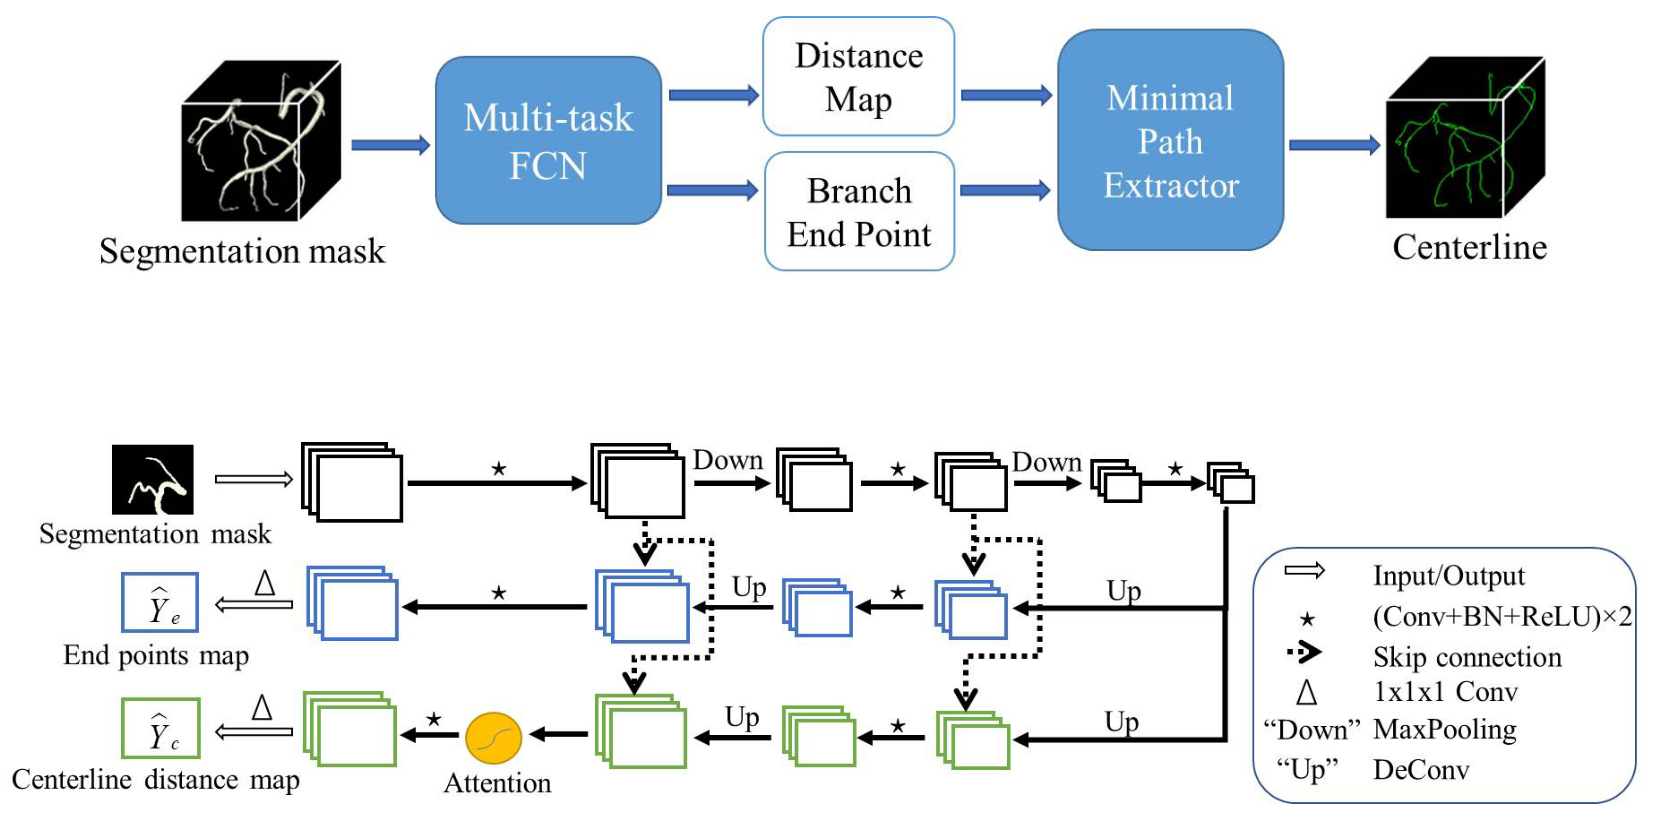
\includegraphics[width=0.8\linewidth]{network-arch-guo.png}
\end{center}
   \caption{Network architecture used by Guo et al. \cite{guoDeepCenterlineMultitaskFully2019} and the base for this work.}
\label{fig:fig1}
\end{figure}

\section{Experiments}



%\begin{figure*}
%\begin{center}
%\fbox{\rule{0pt}{2in} \rule{.9\linewidth}{0pt}}
%%\includegraphics[width=0.8\linewidth]{figure2.pdf}
%\end{center}
%   \caption{Optional detailed illustration of your approach.}
%\label{fig:fig2}
%\end{figure*}

%\begin{table}
%\begin{center}
%\begin{tabular}{c c}
%\hline
%Method & Accuracy \\
%\hline
%Theirs & 0.5 \\
%Yours & 0.75\\
%Ours & \bf 0.9 \\
%\hline
%\end{tabular}
%\end{center}
%\caption{Results for your milestone and final reports.}
%\end{table}


{\small
\bibliography{centerline_bifurcation}
\bibliographystyle{IEEEtran}
}

\end{document}
